\documentclass{article}\usepackage[]{graphicx}\usepackage[]{color}
%% maxwidth is the original width if it is less than linewidth
%% otherwise use linewidth (to make sure the graphics do not exceed the margin)
\makeatletter
\def\maxwidth{ %
  \ifdim\Gin@nat@width>\linewidth
    \linewidth
  \else
    \Gin@nat@width
  \fi
}
\makeatother

\definecolor{fgcolor}{rgb}{0.345, 0.345, 0.345}
\newcommand{\hlnum}[1]{\textcolor[rgb]{0.686,0.059,0.569}{#1}}%
\newcommand{\hlstr}[1]{\textcolor[rgb]{0.192,0.494,0.8}{#1}}%
\newcommand{\hlcom}[1]{\textcolor[rgb]{0.678,0.584,0.686}{\textit{#1}}}%
\newcommand{\hlopt}[1]{\textcolor[rgb]{0,0,0}{#1}}%
\newcommand{\hlstd}[1]{\textcolor[rgb]{0.345,0.345,0.345}{#1}}%
\newcommand{\hlkwa}[1]{\textcolor[rgb]{0.161,0.373,0.58}{\textbf{#1}}}%
\newcommand{\hlkwb}[1]{\textcolor[rgb]{0.69,0.353,0.396}{#1}}%
\newcommand{\hlkwc}[1]{\textcolor[rgb]{0.333,0.667,0.333}{#1}}%
\newcommand{\hlkwd}[1]{\textcolor[rgb]{0.737,0.353,0.396}{\textbf{#1}}}%
\let\hlipl\hlkwb

\usepackage{framed}
\makeatletter
\newenvironment{kframe}{%
 \def\at@end@of@kframe{}%
 \ifinner\ifhmode%
  \def\at@end@of@kframe{\end{minipage}}%
  \begin{minipage}{\columnwidth}%
 \fi\fi%
 \def\FrameCommand##1{\hskip\@totalleftmargin \hskip-\fboxsep
 \colorbox{shadecolor}{##1}\hskip-\fboxsep
     % There is no \\@totalrightmargin, so:
     \hskip-\linewidth \hskip-\@totalleftmargin \hskip\columnwidth}%
 \MakeFramed {\advance\hsize-\width
   \@totalleftmargin\z@ \linewidth\hsize
   \@setminipage}}%
 {\par\unskip\endMakeFramed%
 \at@end@of@kframe}
\makeatother

\definecolor{shadecolor}{rgb}{.97, .97, .97}
\definecolor{messagecolor}{rgb}{0, 0, 0}
\definecolor{warningcolor}{rgb}{1, 0, 1}
\definecolor{errorcolor}{rgb}{1, 0, 0}
\newenvironment{knitrout}{}{} % an empty environment to be redefined in TeX

\usepackage{alltt}

\usepackage{fancyhdr} % Required for custom headers
\usepackage{lastpage} % Required to determine the last page for the footer
\usepackage{extramarks} % Required for headers and footers
\usepackage{graphicx} % Required to insert images
\usepackage{hyperref}
\usepackage{amsmath} %for binomial pdf
\usepackage{parskip} % so that there's space bw paragraphs
\usepackage{float}
\usepackage{amsfonts}
\usepackage{verbatim}
\usepackage{undertilde}
\graphicspath{"~/almhub_0823/exp_design"}



% Margins
\topmargin=-0.45in
\evensidemargin=0in
\oddsidemargin=0in
\textwidth=6.5in
\textheight=9.0in
\headsep=0.25in 

\linespread{1.1} % Line spacing

% Set up the header and footer
\pagestyle{fancy}
\lhead{STAT 541: Experimental Design} % Top left header
\chead{Take Home Mid-term} % Top center header
\rhead{Andrea Mack} % Top right header
\lfoot{02/17/2017} % Bottom left footer
\cfoot{} % Bottom center footer
\rfoot{Page\ \thepage\ of\ \pageref{LastPage}} % Bottom right footer
\renewcommand\headrulewidth{0.4pt} % Size of the header rule
\renewcommand\footrulewidth{0.4pt} % Size of the footer rule

\setlength\parindent{0pt} % Removes all indentation from paragraphs
\setlength\parskip{0.5cm}
\restylefloat{table}

%----------------------------------------------------------------------------------------
%	DOCUMENT STRUCTURE COMMANDS
%	Skip this unless you know what you're doing
%----------------------------------------------------------------------------------------

% Header and footer for when a page split occurs within a problem environment
\newcommand{\enterProblemHeader}[1]{
\nobreak\extramarks{#1}{#1 continued on next page\ldots}\nobreak
\nobreak\extramarks{#1 (continued)}{#1 continued on next page\ldots}\nobreak
}

% Header and footer for when a page split occurs between problem environments
\newcommand{\exitProblemHeader}[1]{
\nobreak\extramarks{#1 (continued)}{#1 continued on next page\ldots}\nobreak
\nobreak\extramarks{#1}{}\nobreak
}


%----------------------------------------------------------------------------------------%
\IfFileExists{upquote.sty}{\usepackage{upquote}}{}
\begin{document}



\begin{enumerate}

\item

\begin{enumerate} %1a
\item

Neither method suggests a transformation.

The Box Cox procedure on the right suggests a transformation of $\hat{\lambda}$ = 1, which does not change the response.

The log standard deviation was regressed on the log mean. There was no evidence the slope differed from 0 indicating (although we do not accept the null hypothesis that the slope is 0) the transformation suggested is 1-0=1, or again, no transformation.

\begin{verbatim}
PROC GLM DATA=yset;
     MODEL logstd=logmean / SS3 solution;
	 run;
\end{verbatim}

\begin{figure}[h!]
\centering
\begin{minipage}{.5\textwidth}
  \centering
  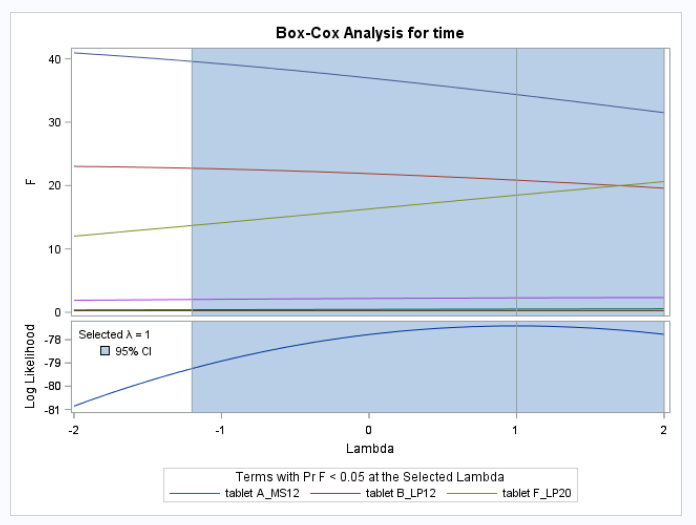
\includegraphics[width=1\linewidth]{prob1a}
  \end{minipage}%
\begin{minipage}{.5\textwidth}
  \centering
  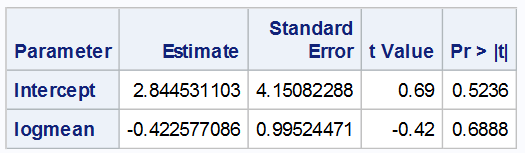
\includegraphics[width=1\linewidth]{prob1a1}
\end{minipage}
\end{figure}
\FloatBarrier


\item 

Let $|\bar{\epsilon_{j}}|$ = the absolute value of true mean error of tablets of type j for j = 1,...,6

$H_{o}$: $|\bar{\epsilon_{1}}| = ... = |\bar{\epsilon_{6}}|$

$H_{a}$: At least one $|\bar{\epsilon_{j}}|$ differs from the rest for j = 1,...,6

Based on a p-value of 0.3874 there is no evidence against the equal variance assumption.

\begin{verbatim}
proc glm data=in1;
class tablet;
model time = tablet /ss3;
means tablet / hovtest=levene(type=abs);
run;
\end{verbatim}

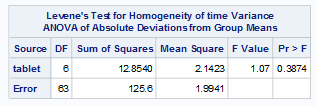
\includegraphics{prob1b}

\item

$y_{ij} = \mu + \tau_{j} + \epsilon_{ij}$

$y_{ij}$ = the ith reponse in the jth tablet type

$\mu$ = the true mean disintegration time averaged over all tablet types in the study

$\tau_{j}$ = the effect of the jth tablet type on the true mean disintegration time

$\epsilon_{ij}$ = the true random error associated with disingetration time of the ith tablet of type j

$\epsilon_{ij} \sim N(0,\sigma^{2})$ and are independent

Two diagnostic plots are below. The standardized residuals fall very close the the associated quantiles from the a standard normal distribution, indicating it is reasonable to assume the residuals follow a normal distribution. Trends are not shown in the residuals vs. fitted plot aside from the grouping by treatment and also because of the randomization, independence in the residuals is reasonable. Based on the test from 1b assessing HOV and on the residuals vs. fitted plot, HOV is reasonable. Although, looking at the scale, we do see a few standardized residuals quite far above the +/- 2 general scope from the empirical rule.

\begin{figure}[h!]
\centering
\begin{minipage}{.5\textwidth}
  \centering
  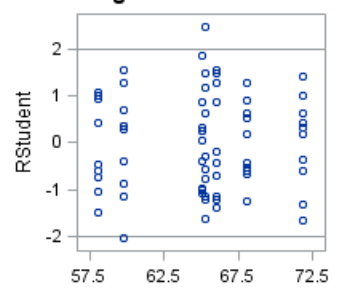
\includegraphics[width=.4\linewidth]{prob1cplots}
  \end{minipage}%
\begin{minipage}{.5\textwidth}
  \centering
  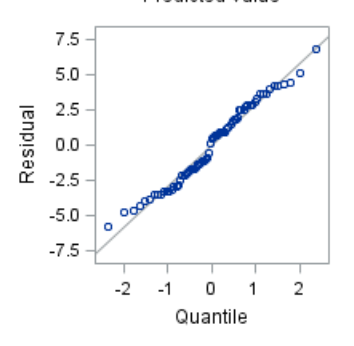
\includegraphics[width=.4\linewidth]{prob1cplots1}
\end{minipage}
\end{figure}

Based on a p-value of \textless 0.001, there is strong evidence at least one of the tablets had a different true mean time to disingetration.

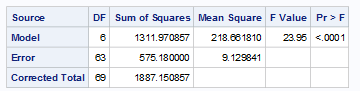
\includegraphics{prob1c}

For the multiple comparisons procedure with G\_TL\_16 as the control, each line of the MC procedure using Dunnett's method is testing:

$H_{o}$: there is no difference in the means between each of the other groups individually (each line is a different group) and the control group (G\_TL\_16)

$H_{a}$: there is a difference in the means between the particular group we are on for that line and the control group

\begin{verbatim}
DATA IN11; 
DO tablet='AZ_MS12', 'B_LP12', 'C_MS16', 'D_LP16', 'E_MS20', 'F_LP20', 'AG_TL_16';
DO rep = 1 TO 10; 
   INPUT time @@; OUTPUT;
END; END;
LINES;
56.3 61.1 60.9 53.8 59.3 56.7 60.8 55.9 60.9 55.1 
57.3 61.8 60.8 63.5 60.6 58.7 56.5 54.1 64.2 60.8 
62.1 63.9 67.5 65.7 65.9 61.9 62.2 65.2 70.2 65.7 
63.6 62.0 64.4 63.1 69.5 68.6 61.8 72.1 60.7 67.1 
69.5 69.8 70.6 68.6 66.3 64.5 66.8 66.1 71.7 66.5 
70.8 74.7 72.3 73.6 73.0 67.1 75.8 72.7 70.1 68.0 
64.7 62.0 65.4 64.0 70.4 69.6 62.7 70.2 62.5 68.5
;
proc glm data=in11;
class tablet;
model time = tablet /ss3;
means tablet / DUNNETT alpha=0.05;
run;
\end{verbatim}


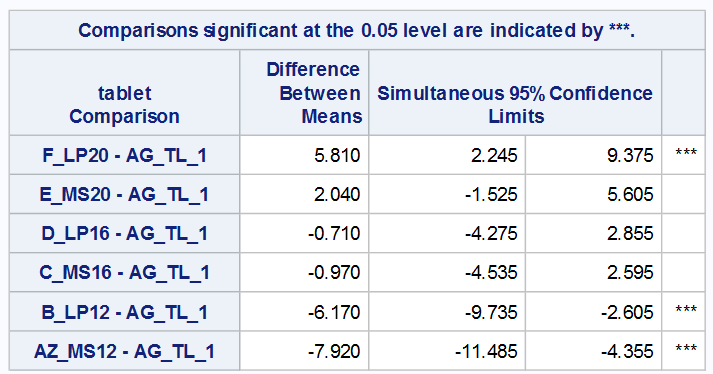
\includegraphics[scale=0.6]{mcdun}

\item 

I did not transform the responses. Normality was reasonable based on the Normal Q-Q plot. The residuals vs. fitted plot showed slight non-constant variance, particularly variation in the D\_LP16 group was slightly larger than the other groups. However, it was not larger by much and may have occured by chance. The HOV assumption was reasonable based on Levene's test. Furthermore, the variation was not increasing as a function of the mean, so standard transformations such as those suggested by the Box Cox method would not fix a non-constant variance assumption. In fact, neither the Box Cox method nor the empirical method suggested a transformation of the response.

\item %1e

{\bf CONTRAST CODE AND OUTPUT (e-h)}

\begin{verbatim}
proc glm data=in1;
class tablet;
model time = tablet;
means / diff;
/* note n = 10 balanced */
contrast 'mean(ms) - mean(lp)' tablet 1/3 -1/3 1/3 -1/3 1/3 -1/3 0;
contrast 'mean(12) - mean(20)' tablet 1/2 1/2 0 0 -1/2 -1/2 0;
contrast 'linear ms' tablet -1 0 0 0 1 0 0;
contrast 'quad ms' tablet  1 0 -2 0 1 0 0;
contrast 'linear lp' tablet 0 -1 0 0 0 1 0;
contrast 'quad lp' tablet 0 1 0 -2 0 1 0;
run;
\end{verbatim}


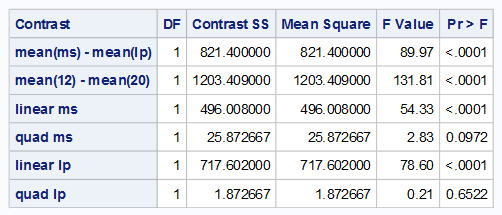
\includegraphics[scale=0.75]{contrast}


{\it  (1.5pt) Perform a test for the contrast comparing the mean of the three disintegration time
means for the magnesium stearate (MS) treatments to the mean of the three disintegration time
means for the three liquid petrolatum (LP) treatments. Be sure to state the hypotheses in terms
of the means (the mui's) and include the associated p-value for the test.}

$H_{0}$: $\frac{1}{3}[\mu_{ams12} + \mu_{cms16} + \mu_{ems20}] = \frac{1}{3}[\mu_{blp12} + \mu_{dlp16} + \mu_{flp20}]$

$H_{a}$: $\frac{1}{3}[\mu_{ams12} + \mu_{cms16} + \mu_{ems20}] \neq \frac{1}{3}[\mu_{blp12} + \mu_{dlp16} + \mu_{flp20}]$

Based on a p-value of \textless 0.0162, there is strong evidence the mean disintegration time of the magesium stearate treatments differed from the mean disintegration time of the liquid petrolatum treatment.

\item
{\it  (1.5pt) The researcher wanted to check for a mesh size effect. To do this, she wants to perform a test for the contrast comparing the mean of the two disintegration time means for the 12 mesh granule size treatments to the mean of the two disintegration time means for the 20 mesh granule size treatments. Be sure to state the hypotheses in terms of the means (the mui's) and include the associated p-value for the test.}

$H_{o}$: $\frac{1}{2}[\mu_{ams12} + \mu_{blp12}] = \frac{1}{2}[\mu_{ems20} + \mu_{fms20}]$

$H_{a}$: $\frac{1}{2}[\mu_{ams12} + \mu_{blp12}] \neq \frac{1}{2}[\mu_{ems20} + \mu_{fms20}]$

Based on a p-value of \textless 0.0001, there is strong evidence the mean disintegration time of the mesh size of 12 treatment differed from the mean disintegration time of the mesh size of 20 treatments.


\item 
{\it  (1.5pt) The researcher wanted to check for linear and quadratic trends for the means across the four granule sizes for the MS tablets. To do this, she wants to use two orthogonal contrasts. Be sure to state the hypotheses in terms of the means (the mui's) and include the associated p-values for the two contrast tests.}

$H_{0}$: $\mu_{ams12} + \mu_{ems20} = \mu_{cms16}$

$H_{a}$: $\mu_{ams12} + \mu_{ems20} \neq \mu_{cms16}$ 

Based on a p-value of \textless 0.0001, there is strong evidence of a linear relationship between mean disintegration time and the mesh size of the magnesium searate treatment.

$H_{0}$: $\frac{1}{2}[\mu_{ams12} + \mu_{ems20}] = \mu_{cms16}$

$H_{a}$: $\frac{1}{2}[\mu_{ams12} + \mu_{ems20}] \neq \mu_{cms16}$ 

Based on a p-value of 0.0972, there is some evidence of a quadratic relationship between mean disintegration time and mesh size in the magnesium searate treatment.


\item
{\it  (1.5pt) The researcher wanted to check for linear and quadratic trends for the means across the four granule sizes for the LP tablets. To do this, she wants to use two orthogonal contrasts. Be sure to state the hypotheses in terms of the means (the mui's) and include the associated p-values for the two contrast tests.}

$H_{0}$: $\mu_{blp12} + \mu_{dlp20} = \mu_{flp16}$

$H_{a}$: $\mu_{blp12} + \mu_{dlp20} \neq \mu_{flp16}$

Based on a p-value of \textless 0.0001, there is strong evidence of a linear relationship between the mean disintegration time and the mesh size in the liquid petrolatum treatment.

$H_{0}$: $\frac{1}{2}[\mu_{blp12} + \mu_{dlp20}] = \mu_{flp16}$

$H_{a}$: $\frac{1}{2}[\mu_{blp12} + \mu_{dlp20}] \neq \mu_{flp16}$

Based on a p-value of 0.6522, there is no evidence of a quadratic relationship between mean disintegration time and the mesh size in the liquid petrolatum treatment. 


\item 
{\it (1.5pt) Compare the results of the orthogonal contrasts in (g) and (h) to the side-by-side boxplots. Briefly describe why the contrast results are or are not consistent with the pattern of the boxplots.}


{\bf DRAW LINES IN BOXPLOTS AND DISCUSS}


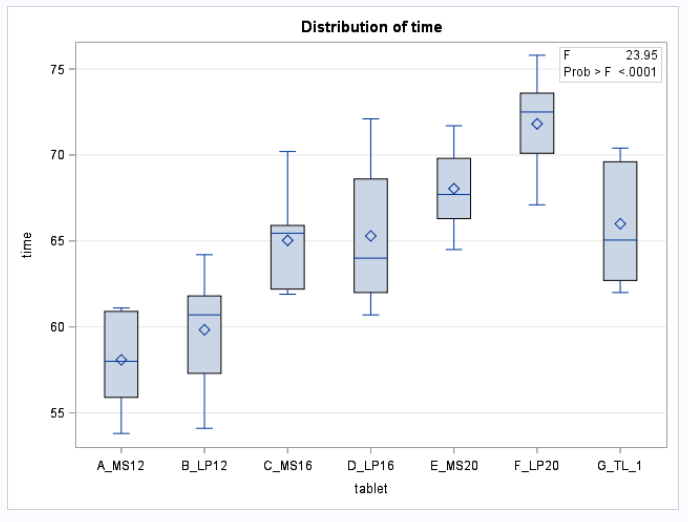
\includegraphics[scale=0.5]{boxplots}


\end{enumerate}

\item %2
{\bf PROBLEM 2 SAS CODE}
\begin{verbatim}

proc glm data=in;
class glass subject;
model guess= subject glass;
random subject;
contrast 'mean(s) - mean(b)' glass 1 -1 -1 0 1 0;
contrast 'mean(others) - mean(tea)' glass 1 1 1 1 1 -5;
run;
\end{verbatim}

{\bf REDO WITH BLOCKING VARIABLE FIRST}

\begin{enumerate}
\item 
{\it  (6.5pt) Perform a complete analysis comparing the means of the student guesses. Be sure you include the model and state all hypotheses tested. Also include Bonferroni's multiple comparison test. You do not need to transform the response. Use $\alpha$ = .10 for testing.}

Let i = 1,...,6 and j = 1,...,15

$Y_{ij} = \mu + \tau_{i} + \utilde{\beta}_{j} + \utilde{\epsilon}_{ij}$

$Y_{ij}$ = the guess in ounces of student j for glass i

$\mu$ = the true mean guess in ounces averaged over all students and all glasses

$\tau_{i}$ = the true change in mean guess for glass i from the overall mean guess averaged over all students

$\utilde{\beta}_{j} \sim N(0,\sigma^{2}_{b})$ = the random effect associated with student j, where students are assumed independent of one another and of the random error ($\utilde{\epsilon}_{ij}$)

$\utilde{\epsilon}_{ij} \sim N(0,\sigma^{2})$ = the random error associated with guess i from student j, where each $\epsilon}_{ij}$ is assumed to be independent of all others and independent of the random student effect ($\utilde{\beta}_{j}$)

$H_{o}$: $\tau_{1} = ... = \tau_{6}$

$H_{a}$: at least one $\tau_{i} \neq \tau_{i'}$ among all i $\neq$ i' for i in 1,...,6

Based on a p-value of \textless 0.0001, after accounting for variation among students, there is strong evidence the mean guesses were different for at least two glasses.

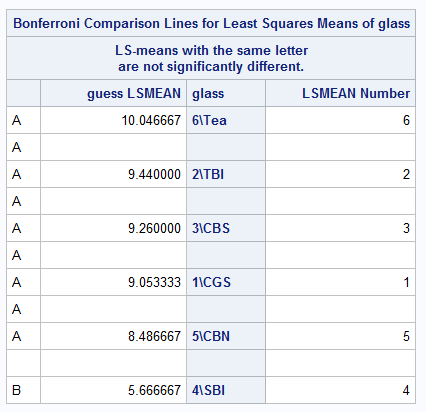
\includegraphics{cldglasses}

Based on the Bonferroni correction for multiple comparisons, at the family-wise $\alpha$ = 0.1 significance threshold, there is strong evidence that the true mean guess for glass SBI differed from the true mean guess for all other glasses. There was no evidence of a difference in true mean guess between all other glasses at the 90\% family-wise Bonferroni adjusted confidence level.

{\bf ASSESSING MODEL ASSUMPTIONS}

The HOV assumption is likely violated as the studentized error residuals vs. fitted plot shows increasing variance with increasing mean. Normality in error residuals appears reasonable to assume as the residuals fall close to the line based on theoretical normal quantiles.

\begin{figure}
\centering
\begin{minipage}{.5\textwidth}
  \centering
  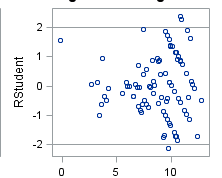
\includegraphics[width=.6\linewidth]{glasshov}
  \end{minipage}%
\begin{minipage}{.5\textwidth}
  \centering
  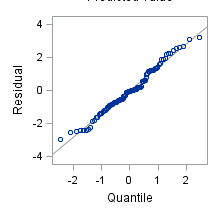
\includegraphics[width=.6\linewidth]{glassnorm}
\end{minipage}
\end{figure}

It is reasonable to assume the variation is the same within each subject.

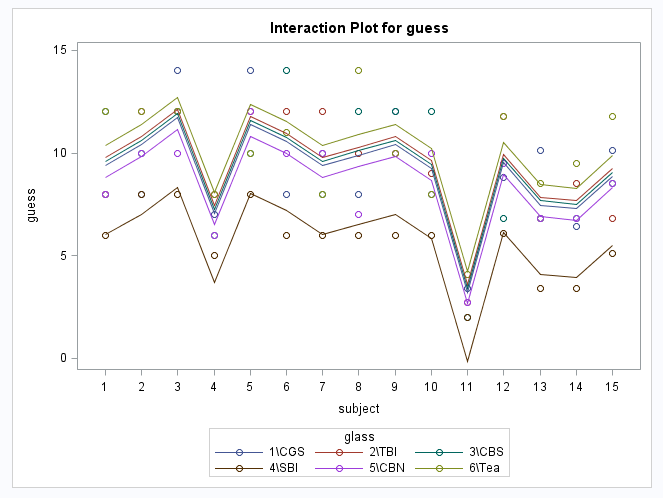
\includegraphics[scale=0.75]{level2}

Glass placement order was not randomized, so there may be a carry-over effect within each subject, making observations within each subject not independent. Unless students looked at each others' answers, it is reasonable to believe that students' guesses were independent. We also assume random errors in guesses do not depend on random student effects around the overall mean guess.


\item %2b
{\it  (1.5pt) Perform a test for the contrast comparing the mean of the two means for the stemmed
glasses to the mean of the two means for the blue glasses. Be sure to include the p-value.}

Based on a p-value of 0.0002, there is strong evidence of a difference in mean guess between the stemmed and blue glasses.

\begin{verbatim}proc glm data=in;
class glass subject;
model guess= subject glass;
random subject;
contrast 'mean(s) - mean(b)' glass 1 -1 1 -1 0 0;
contrast 'mean(others) - mean(tea)' glass 1 1 1 1 1 -5;
run;
\end{verbatim}

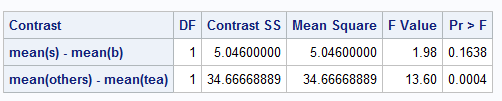
\includegraphics[scale=0.75]{contrastp2}

\item %2c
{\it  (1.5pt) Perform a test for the contrast comparing the tea mug mean to the mean of the five means for the other glasses. Be sure to include the p-value.}

Based on a p-value of 0.0004, there is strong evidence of a different in the mean tea guess and between the mean of guesses of all other glasses.

\item 

The contrasts are orthoganol because the sum of the coefficients is 0 in both cases.

\item 
{\it  (2pt) Suppose you are asked to compare how close the guesses were to the true glass volumes
across the six glass treatments. Briefly describe how (if possible) you could address this request
from the data provided. No analysis is required. If you do not believe this can be addressed,
briefly give a reason why.}

Yes, this can be addressed. The {\bf null} hypotheses change to:

1) $\mu_{2TBI} = 9$

2) $\mu_{3CBS} = 9$

3) $\mu_{4TEA} = 9$

4) $\mu_{5SBI} = 9$

5) $\mu_{1CGS} = 10$

6) $\mu_{6CBN} = 11$

I would create confidence intervals and see whether the true value was in the confidence interval for each mean. We can adjust for multiple comparisons if that is necessary.

\end{enumerate}

\item 
{\it  (2.5pt) Look at the attached SAS output. It contains two ANOVA tables. On the top is the ANOVA
for a RCBD and on the bottom is the ANOVA for the RCBD data but with blocks removed from the
model. At an $\alpha$ = .05 level, you would draw different conclusions regarding the equality of treatment effects. Suppose you hear the following: ``By systematically controlling outside effects, the residual mean square error will be reduced.
This increases the precision of the experiment making detection of significant effects
more likely." This example may appear to be inconsistent this statement. Explain why you reject the null hypothesis without blocks and fail to reject the null hypothesis with blocks (assuming $\alpha$ = .05).
}

The sums of squares associated with the blocking variable do not explain enough variation in the model to ``pay off" for the additional number of parameters that need to be estimated to include block in the model.

\item
{\it Use the sample means and an estimate of $\sigma$ based on the oneway ANOVA to estimate the sample
size needed for a CRD to achieve}

Note the estimate of $\sigma$ = sqrt(46.9054167) = 6.8487529 which is the RMSE from the one way ANOVA.

\begin{verbatim}
PROC GLMPOWER DATA = p4;
CLASS nitrogen;
MODEL yield=nitrogen;
POWER
STDDEV = 6.848753
ALPHA = 0.05 0.10
NTOTAL = .
POWER = 0.7 0.71 0.72 0.73 0.74 0.75 0.8 0.85 0.9 0.91 0.92 0.93 0.94 0.95;
TITLE 'Power Calc';
RUN;
\end{verbatim}

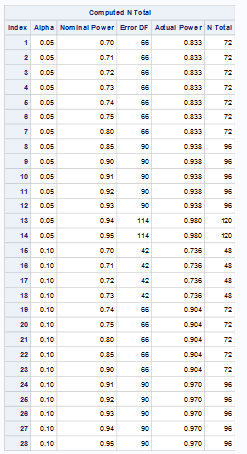
\includegraphics{power}

\begin{enumerate}
\item
{\it  A power of at least .95 for the ANOVA F-test assuming $\alpha$ = .05.}

N = 120 or 20 observations per nitrogen treatment with a balanced design will give a power of 0.98

\item 
{\it A power of at least .90 for the ANOVA F-test assuming $\alpha$ = .01.}

N = 72 or 12 observations per nitrogen treatment with a balanced design will give a power of 0.94

\item
{\it What would be the estimated power for the ANOVA F-test assuming n = 2 replicates are to be taken for each treatment and assuming $\alpha$ = .05?}

Two replicates per group is not enough to detect a difference and so the power cannot be estimated.

\begin{verbatim}
PROC GLMPOWER DATA = p4;
CLASS nitrogen;
MODEL yield=nitrogen;
POWER
STDDEV = 6.848753
ALPHA = 0.05
NTOTAL = 18 24 36 48
POWER = .;
TITLE 'Power Calc';
RUN;
\end{verbatim}

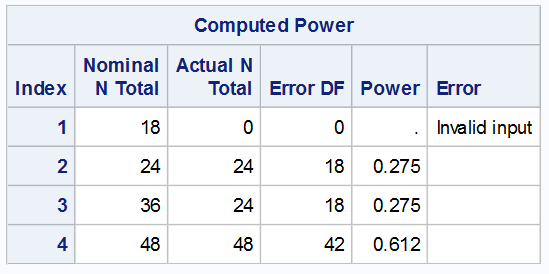
\includegraphics{power2}


\end{enumerate}


\item %5
{\it  (5pt) Stat 541 Students: Read Section 4.3 (pages 165-168) on Graeco-Latin squares. Consider the
following experiment. A food processor wants to determine the effect of package design on the sale of
one of her company's products. She had five designs to be tested: A, B, C, D, E. There were several
sources of variation, however, whose possible effects were to be accounted for in the study. These
included (1) day of the week, (2) differences among stores, and (3) effect of shelf height. She decided
to use a Graeco-Latin square with five weekdays (M, Tu, W, Th, F,) for the row blocks, five stores
for the column blocks, and five shelf heights for the Greek letter blocks. The experimental design
and sales in dollars are shown in the following table.
}

\begin{knitrout}\footnotesize
\definecolor{shadecolor}{rgb}{0.969, 0.969, 0.969}\color{fgcolor}\begin{kframe}
\begin{alltt}
\hlcom{# create latin squares data set}

\hlstd{rowsday} \hlkwb{<-} \hlkwd{c}\hlstd{(}\hlkwd{rep}\hlstd{(}\hlkwd{c}\hlstd{(}\hlstr{"Mon"}\hlstd{,} \hlstr{"Tues"}\hlstd{,} \hlstr{"Wed"}\hlstd{,} \hlstr{"Thurs"}\hlstd{,} \hlstr{"Fri"}\hlstd{),}\hlnum{5}\hlstd{))}
\hlstd{colstore} \hlkwb{<-} \hlkwd{c}\hlstd{(}\hlkwd{rep}\hlstd{(}\hlstr{"I"}\hlstd{,} \hlnum{5}\hlstd{),} \hlkwd{rep}\hlstd{(}\hlstr{"II"}\hlstd{,} \hlnum{5}\hlstd{),} \hlkwd{rep}\hlstd{(}\hlstr{"III"}\hlstd{,} \hlnum{5}\hlstd{),}
              \hlkwd{rep}\hlstd{(}\hlstr{"IV"}\hlstd{,} \hlnum{5}\hlstd{),} \hlkwd{rep}\hlstd{(}\hlstr{"V"}\hlstd{,} \hlnum{5}\hlstd{))}
\hlstd{latin} \hlkwb{<-} \hlkwd{c}\hlstd{(}\hlstr{"E"}\hlstd{,} \hlstr{"D"}\hlstd{,} \hlstr{"B"}\hlstd{,} \hlstr{"C"}\hlstd{,} \hlstr{"A"}\hlstd{,} \hlstr{"C"}\hlstd{,} \hlstr{"B"}\hlstd{,} \hlstr{"E"}\hlstd{,} \hlstr{"A"}\hlstd{,} \hlstr{"D"}\hlstd{,}
           \hlstr{"B"}\hlstd{,} \hlstr{"A"}\hlstd{,} \hlstr{"D"}\hlstd{,} \hlstr{"E"}\hlstd{,} \hlstr{"C"}\hlstd{,}\hlstr{"A"}\hlstd{,} \hlstr{"E"}\hlstd{,} \hlstr{"C"}\hlstd{,} \hlstr{"D"}\hlstd{,} \hlstr{"B"}\hlstd{)}

\hlstd{greek} \hlkwb{<-} \hlkwd{c}\hlstd{(}\hlstr{"alpha"}\hlstd{,} \hlstr{"delta"}\hlstd{,} \hlstr{"epsilon"}\hlstd{,} \hlstr{"beta"}\hlstd{,} \hlstr{"gamma"}\hlstd{,} \hlstr{"delta"}\hlstd{,}
           \hlstr{"beta"}\hlstd{,} \hlstr{"gamma"}\hlstd{,} \hlstr{"epsilon"}\hlstd{,} \hlstr{"alpha"}\hlstd{,} \hlstr{"gamma"}\hlstd{,} \hlstr{"alpha"}\hlstd{,}
           \hlstr{"beta"}\hlstd{,} \hlstr{"delta"}\hlstd{,} \hlstr{"epsilon"}\hlstd{,} \hlstr{"epsilon"}\hlstd{,} \hlstr{"gamma"}\hlstd{,} \hlstr{"delta"}\hlstd{,}
           \hlstr{"alpha"}\hlstd{,} \hlstr{"beta"}\hlstd{,} \hlstr{"beta"}\hlstd{,} \hlstr{"epsilon"}\hlstd{,} \hlstr{"alpha"}\hlstd{,} \hlstr{"gamma"}\hlstd{,} \hlstr{"delta"}\hlstd{)}

\hlstd{dollars} \hlkwb{<-} \hlkwd{c}\hlstd{(}\hlnum{238}\hlstd{,}\hlnum{149}\hlstd{,}\hlnum{222}\hlstd{,}\hlnum{187}\hlstd{,}\hlnum{65}\hlstd{,}\hlnum{228}\hlstd{,}\hlnum{220}\hlstd{,}\hlnum{295}\hlstd{,}\hlnum{66}\hlstd{,}\hlnum{118}\hlstd{,}\hlnum{158}\hlstd{,}\hlnum{92}\hlstd{,}\hlnum{104}\hlstd{,}\hlnum{242}\hlstd{,}
             \hlnum{279}\hlstd{,}\hlnum{188}\hlstd{,}\hlnum{169}\hlstd{,}\hlnum{54}\hlstd{,}\hlnum{122}\hlstd{,}\hlnum{278}\hlstd{,}\hlnum{74}\hlstd{,}\hlnum{282}\hlstd{,}\hlnum{213}\hlstd{,}\hlnum{90}\hlstd{,}\hlnum{176}\hlstd{)}

\hlstd{p5data} \hlkwb{<-} \hlkwd{data.frame}\hlstd{(}\hlkwd{cbind}\hlstd{(rowsday, colstore, latin, greek, dollars))}
\end{alltt}


{\ttfamily\noindent\color{warningcolor}{Warning in cbind(rowsday, colstore, latin, greek, dollars): number of rows of result is not a multiple of vector length (arg 3)}}\begin{alltt}
\hlkwd{dim}\hlstd{(p5data)}
\end{alltt}
\begin{verbatim}
[1] 25  5
\end{verbatim}
\begin{alltt}
\hlkwd{aggregate}\hlstd{(}\hlkwd{as.numeric}\hlstd{(}\hlkwd{as.character}\hlstd{(p5data}\hlopt{$}\hlstd{dollars)),} \hlkwd{list}\hlstd{(}\hlkwd{as.factor}\hlstd{(p5data}\hlopt{$}\hlstd{rowsday)), mean)}
\end{alltt}
\begin{verbatim}
  Group.1     x
1     Fri 183.2
2     Mon 177.2
3   Thurs 141.4
4    Tues 182.4
5     Wed 177.6
\end{verbatim}
\begin{alltt}
\hlcom{#write.csv(p5data, file = "p5data.csv")}

\hlstd{mon} \hlkwb{<-} \hlkwd{c}\hlstd{(}\hlnum{238}\hlstd{,}\hlnum{228}\hlstd{,}\hlnum{158}\hlstd{,}\hlnum{188}\hlstd{,}\hlnum{74}\hlstd{)}
\hlstd{tues} \hlkwb{<-} \hlkwd{c}\hlstd{(}\hlnum{149}\hlstd{,}\hlnum{220}\hlstd{,}\hlnum{92}\hlstd{,}\hlnum{169}\hlstd{,}\hlnum{282}\hlstd{)}
\hlstd{wed} \hlkwb{<-} \hlkwd{c}\hlstd{(}\hlnum{222}\hlstd{,}\hlnum{295}\hlstd{,}\hlnum{104}\hlstd{,}\hlnum{54}\hlstd{,}\hlnum{213}\hlstd{)}
\hlstd{thurs} \hlkwb{<-} \hlkwd{c}\hlstd{(}\hlnum{187}\hlstd{,}\hlnum{66}\hlstd{,}\hlnum{242}\hlstd{,}\hlnum{122}\hlstd{,}\hlnum{90}\hlstd{)}
\hlstd{fri} \hlkwb{<-} \hlkwd{c}\hlstd{(}\hlnum{65}\hlstd{,}\hlnum{118}\hlstd{,}\hlnum{279}\hlstd{,}\hlnum{278}\hlstd{,}\hlnum{176}\hlstd{)}
\hlkwd{c}\hlstd{(}\hlkwd{mean}\hlstd{(mon),} \hlkwd{mean}\hlstd{(tues),} \hlkwd{mean}\hlstd{(wed),} \hlkwd{mean}\hlstd{(thurs),} \hlkwd{mean}\hlstd{(fri))}
\end{alltt}
\begin{verbatim}
[1] 177.2 182.4 177.6 141.4 183.2
\end{verbatim}
\end{kframe}
\end{knitrout}

\begin{enumerate}
\item
{\it Perform an ANOVA. State the null and alternative hypotheses of interest, and your conclusions.
You can use $\alpha$ = .05 for testing.}

$Y_{ijkl} = \mu + \beta_{i} + \gamma_{j} + \psi_{k} + \tau_{l} + \epsilon_{ijkl}$

Let $\tau_{l}$ represents the effect of design l which is an element of the set A,B,C,D,E.

$H_{o}$: $\tau_{A} = \tau_{B} = \tau_{C} = \tau_{D} = \tau_{E}$

$H_{a}$: at least one $\tau_{l} \neq \tau_{l'}$ for $l \neq l'$

Based on a p-value of 0.2828, there is no evidence of a design effect on the true mean price. At the $\alpha$ =  0.05 cutoff, the design did not have an effect on the true mean price after accounting for the store, shelf, and weekday effects.

\begin{verbatim}
proc glm data=p5data; 
title 'Graeco-Latin Square';
class rowsday colstore latin greek;
model newdollar = rowsday colstore latin greek;
means latin / tukey alpha=0.05;
run;
\end{verbatim}

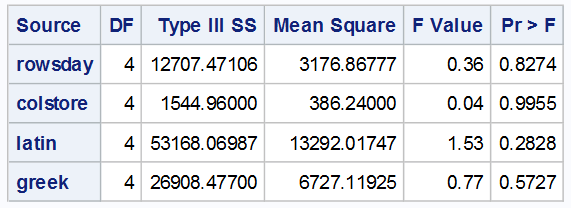
\includegraphics{latin}


\item
{\it  Include a Tukey multiple comparison procedure, and your conclusions from it.}

Using the 95\% Tukey adjusted family-wise confidence level, there is no evidence the mean cost differs for any of the designs.

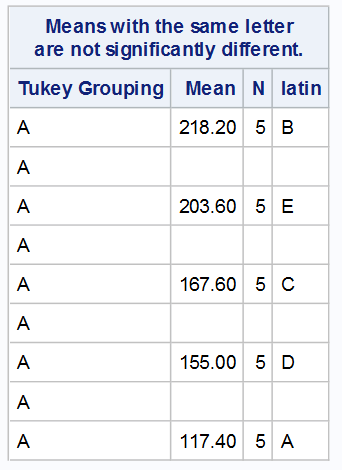
\includegraphics{latintuk}

\end{enumerate}

\item

See attached.
\end{enumerate}
\end{document}
